\documentclass[10pt]{article}
\usepackage[polish]{babel}
\usepackage[utf8]{inputenc}
\usepackage[T1]{fontenc}
\usepackage{amsmath}
\usepackage{amsfonts}
\usepackage{amssymb}
\usepackage[version=4]{mhchem}
\usepackage{stmaryrd}
\usepackage{graphicx}
\usepackage[export]{adjustbox}
\graphicspath{ {./images/} }

\title{KLASY PO SZKOLE PODSTAWOWEJ }

\author{}
\date{}


\newcommand\Varangle{\mathop{{<\!\!\!\!\!\text{\small)}}\:}\nolimits}

\begin{document}
\maketitle
\begin{enumerate}
  \item Dany jest czworokąt wypukły \(A B C D, w\) którym \(\Varangle D A B=\Varangle A B C\). Symetralne odcinków AD i BC przecinają się w punkcie M leżącym na odcinku \(A B\). Udowodnij, że \(A C=B D\).
  \item Na przeciwprostokątnej \(B C\) trójkąta prostokątnego \(A B C\) zbudowano po zewnętrznej stronie kwadrat BCDE. Niech O będzie środkiem tego kwadratu. Wykazać, że \(\Varangle B A O=\Varangle C A O\).
  \item Czy istnieje taki trójkąt o bokach długości \(a, b, c\), którego pole jest równe \(\frac{a b+b c}{4}\) ? Odpowiedź uzasadnij.\\
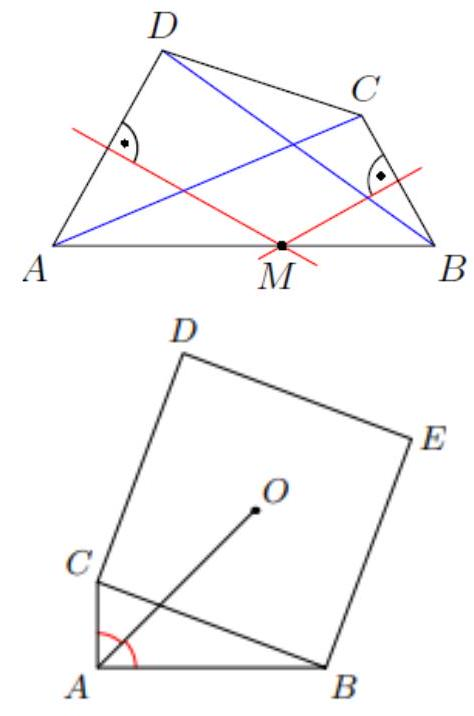
\includegraphics[max width=\textwidth, center]{2024_11_21_c9a6645e9f491eb56f73g-1(1)}
\end{enumerate}

\section*{KLASY PO GIMNAZJUM}
\begin{enumerate}
  \item Udowodnij, używając twierdzenia Ptolemeusza, że w pięciokącie foremnym przekątna i bok pozostają w złotej proporcji, czyli, że ich stosunek wynosi \(\frac{1+\sqrt{5}}{2}\).
  \item Na przeciwprostokątnej \(A B\) trójkąta prostokątnego \(A B C\) zbudowano, po jego wewnętrznej stronie, kwadrat ABDE o środku O. Znając długości odcinków AC i BC oblicz długość odcinka OC.
  \item Dany jest trójkąt \(A B C\), w którym spełniona jest równość \(A C+B C=2 A B\). Punkt I jest środkiem okręgu wpisanego w trójkąt \(A B C\), a punkt \(O\) jest środkiem okręgu opisanego na tym trójkącie. Wykaż, że jeżeli \(\mathrm{O} \neq \mathrm{I}\), to proste OI i Cl są prostopadłe.\\
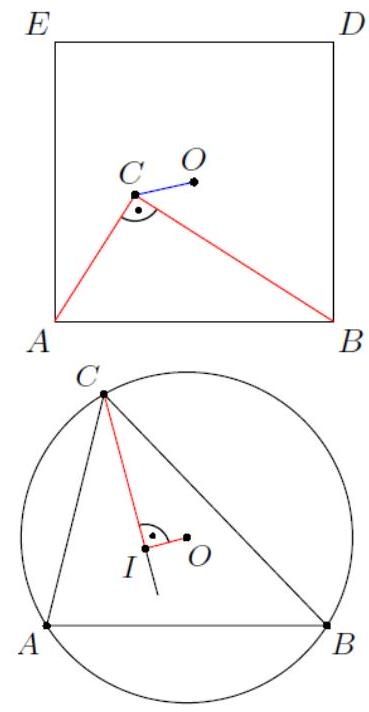
\includegraphics[max width=\textwidth, center]{2024_11_21_c9a6645e9f491eb56f73g-1}
\end{enumerate}

\end{document}